\documentclass[14pt,a4paper]{extarticle}
\pagestyle{empty}
\usepackage{fontspec}
\usepackage{polyglossia}
\setmainlanguage{ukrainian}
\IfFontExistsTF{Times New Roman}{\setmainfont{Times New Roman}\newfontfamily\ukrainianfont{Times New Roman}}{\setmainfont{Libertinus Serif}\newfontfamily\ukrainianfont{Libertinus Serif}}
\IfFontExistsTF{Courier New}{\setmonofont{Courier New}\newfontfamily\ukrainianfonttt{Courier New}}{\setmonofont{DejaVu Sans Mono}\newfontfamily\ukrainianfonttt{DejaVu Sans Mono}}
\usepackage[top=20mm,bottom=20mm,left=25mm,right=15mm]{geometry}
\usepackage{setspace,indentfirst,graphicx,float,caption,enumitem,titlesec,tikz}
\usetikzlibrary{arrows.meta,positioning}
\onehalfspacing
\setlength{\parindent}{1.25cm}
\setlength{\parskip}{0pt}
\captionsetup{font=it,justification=centering}
\titleformat{\section}{\normalfont\normalsize\bfseries\centering}{}{0pt}{}
\titlespacing*{\section}{0pt}{0.8\baselineskip}{0.4\baselineskip}
\graphicspath{{images/}}
\begin{document}
\begin{titlepage}
\begin{center}
Міністерство освіти і науки України

Національний університет «Львівська політехніка»

\vspace{0.7cm}

\includegraphics[height=7cm]{logo.png}

\vspace{1cm}
\textbf{Звіт до лабораторної роботи №2}

з дисципліни

«Програмування мобільних додатків»

на тему

«Базова реалізація мобільного AI-застосунку»
\vspace{1.5cm}
\end{center}
\begin{flushright}
Виконав:\\студент групи АП-41\\Чижевський М. М.\\[1cm]
Прийняв:\\доц. каф. ІКТ, докт. ф.\\Андрущак В. С.
\end{flushright}
\vfill
\begin{center}Львів 2026\end{center}
\end{titlepage}

\section*{Мета роботи}
Реалізувати один робочий сценарій Ohmlette з передаванням даних через HTTP, обробкою на backend та поверненням результату в Android-додаток.

\section*{Хід роботи}
У цій роботі я реалізував створення чернетки картки даташита. На екрані «Даташити» користувач вводить адресу сервера, артикул і посилання на PDF або вибирає файл із пристрою. Після натискання «Створити картку» додаток надсилає запит на сервер.

Android-частину написано на Kotlin із Jetpack Compose, backend — на Python. Для читання PDF використав pypdf. Сервер перевіряє вхідні дані, обмежує розмір файла до 15 МіБ та кількість сторінок до 100. Якщо файл не містить тексту або його неможливо прочитати, повертається повідомлення про помилку.

\begin{figure}[H]
\centering
\begin{tikzpicture}[
block/.style={draw=black!60,rounded corners=3pt,fill=black!3,
text width=11cm,align=center,inner sep=7pt,font=\small},
flow/.style={<->,>=Latex,line width=0.7pt}]
\node[block] (app) {\textbf{Android · Ohmlette}\\Артикул і PDF → запит → картка або помилка};
\node[block,below=0.8cm of app] (api) {\textbf{HTTP API · Python}\\Перевірка даних → читання PDF → пошук фрагментів};
\node[block,below=0.6cm of api] (ai) {\textbf{AI-класифікатор · Naive Bayes}\\Визначення типу компонента за текстом};
\draw[flow] (app) -- node[right,font=\small]{JSON} (api);
\draw[flow] (api) -- (ai);
\end{tikzpicture}
\caption{Схема обміну даними}
\end{figure}

AI-компонентом є простий класифікатор Naive Bayes, навчений на невеликому наборі текстових прикладів. Він розрізняє діоди, резистори, конденсатори та дроселі. Це не мовна модель: знайдені фрагменти витягуються з PDF окремо, а картка позначається як неперевірена.

\clearpage
\section*{Перевірка застосунку}
Я запустив Ohmlette на емуляторі Medium Phone API 37.0, а backend — на ПК, порт 8000. Для з'єднання використав перенаправлення порту командою \texttt{adb reverse tcp:8000 tcp:8000}. У застосунку вказав \texttt{http://127.0.0.1:8000}.

Для перевірки обрав даташит onsemi та артикул BZX84C2V4LT1G. На рисунку 2 показано заповнену форму. Щоб перевірити оброблення помилок, я тимчасово змінив порт на 8001. Застосунок показав помилку з'єднання й залишив можливість повторити запит.

\begin{figure}[H]
\centering
\begin{minipage}[t]{0.47\textwidth}
\centering
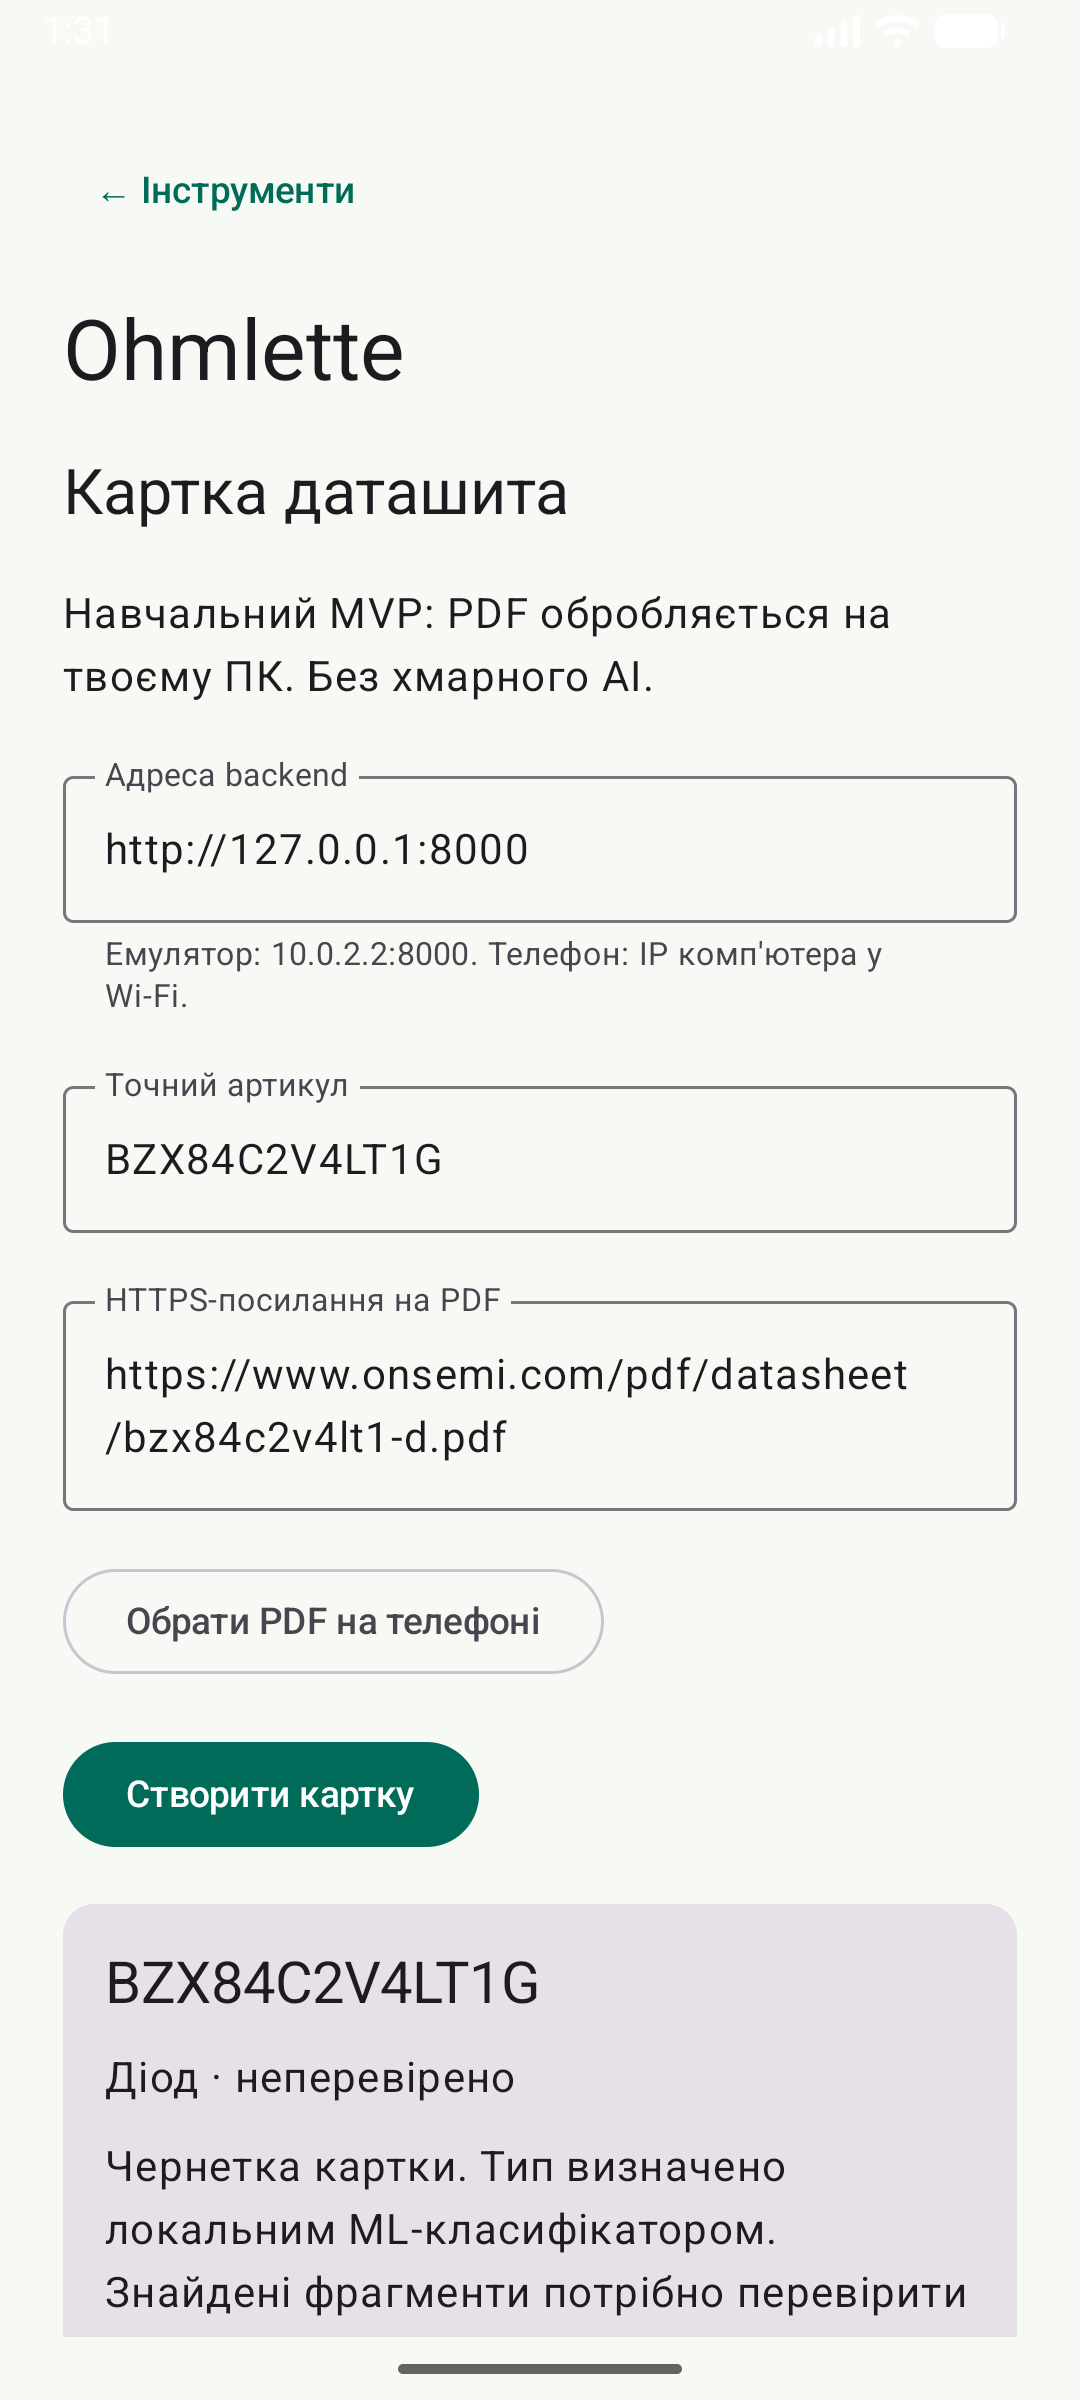
\includegraphics[width=\linewidth,height=13.5cm,keepaspectratio]{s1_lab2.png}
\caption{Введення даних}
\end{minipage}\hfill
\begin{minipage}[t]{0.47\textwidth}
\centering
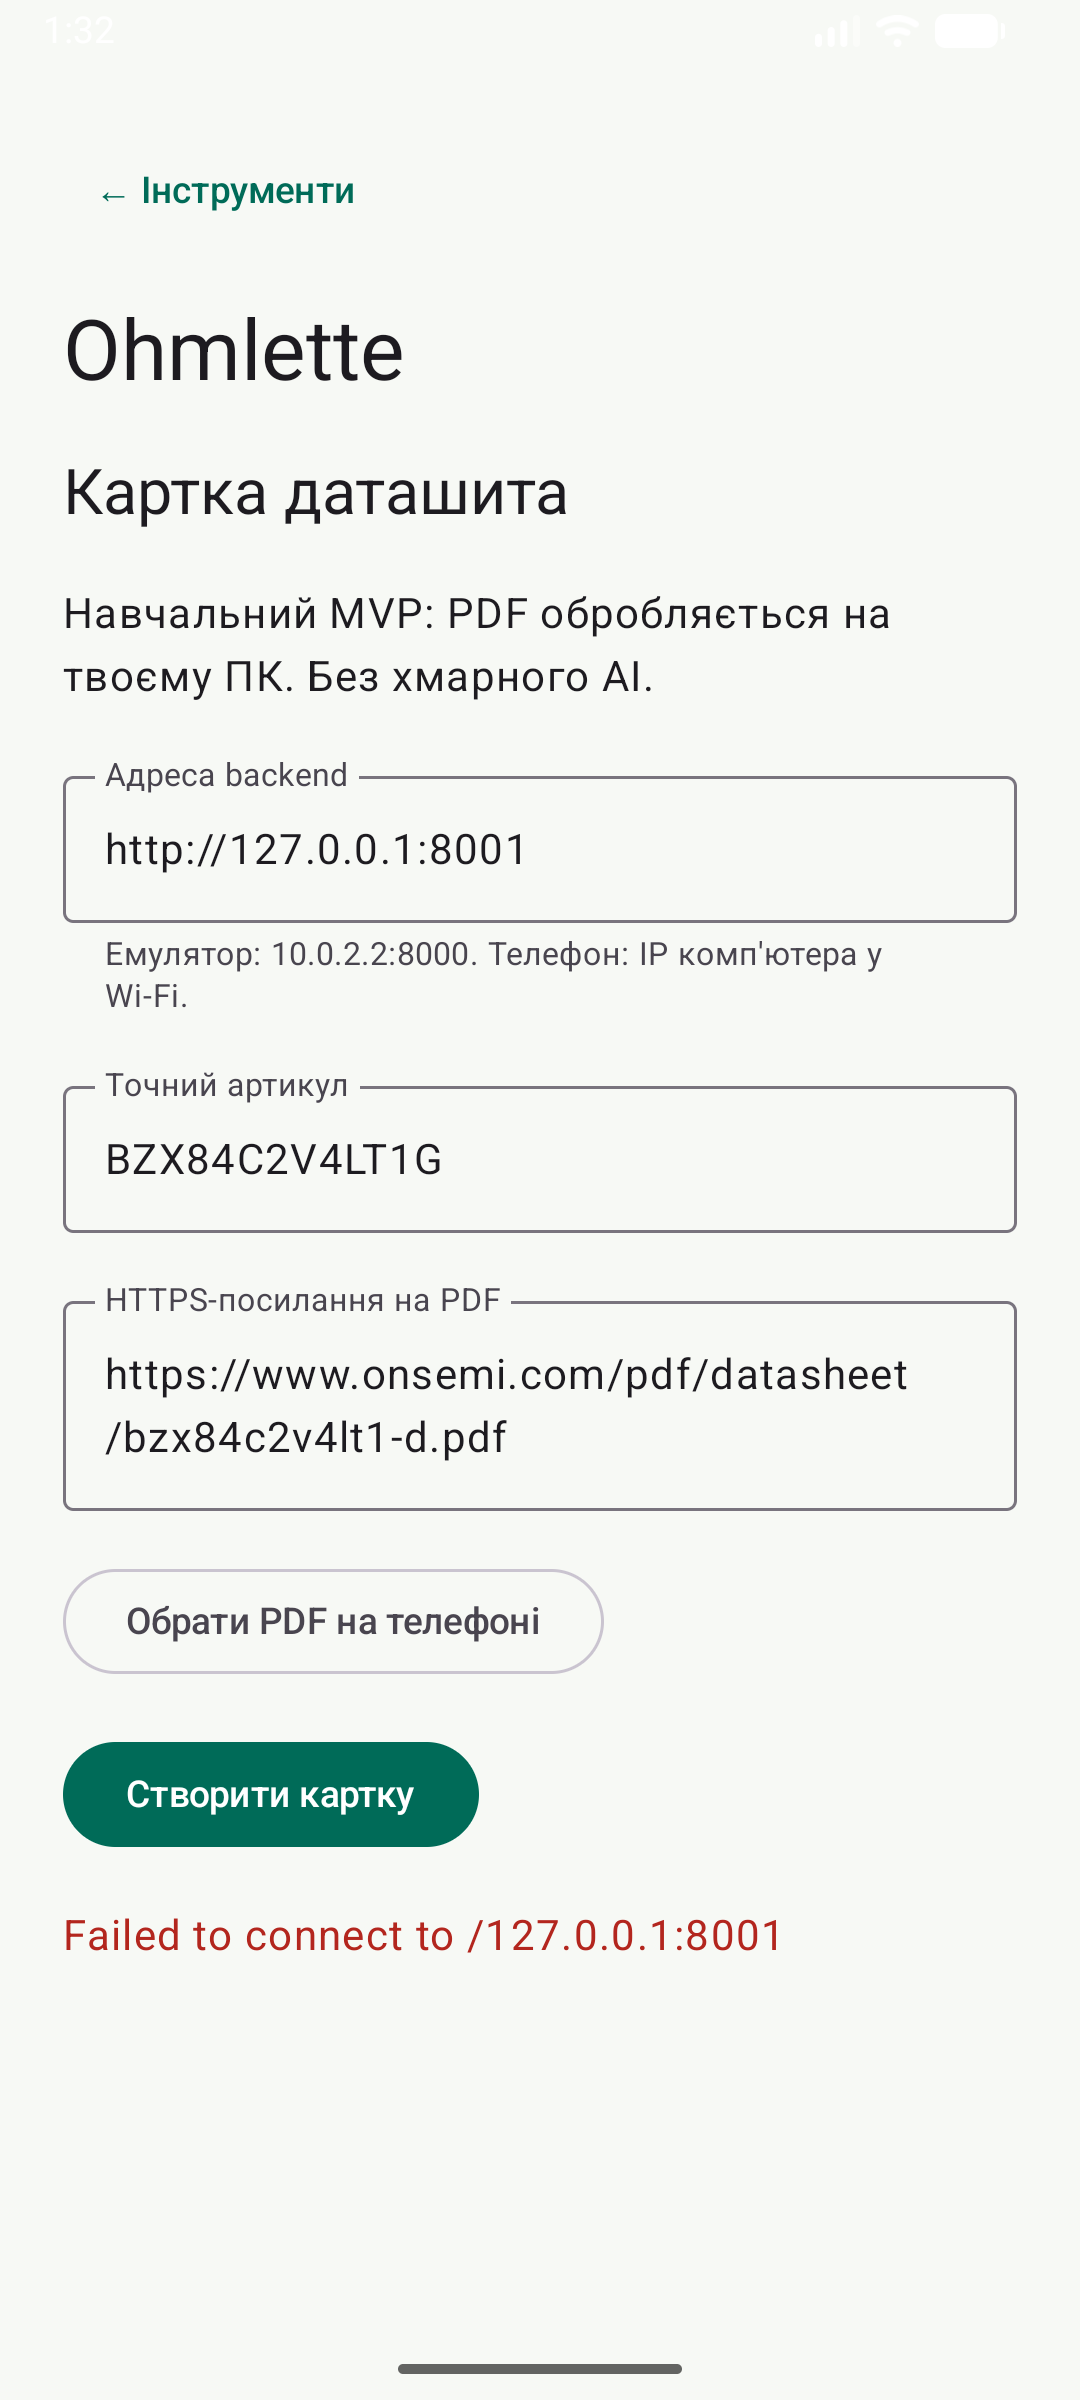
\includegraphics[width=\linewidth,height=13.5cm,keepaspectratio]{s3_lab2.png}
\caption{Помилка з'єднання}
\end{minipage}
\end{figure}

Після повернення порту 8000 я повторив запит і знову отримав картку. Таким чином перевірив успішне з'єднання та поведінку при недоступному сервері.

\clearpage
\section*{Результат}
Сервер визначив тип компонента як «Діод» і повернув фрагмент зі сторінки 3, де є вказаний артикул. Додаток відобразив результат і номер сторінки. Поки що картка містить оригінальний текст: значення min/typ/max та умови не розбираються автоматично.

\begin{figure}[H]
\centering
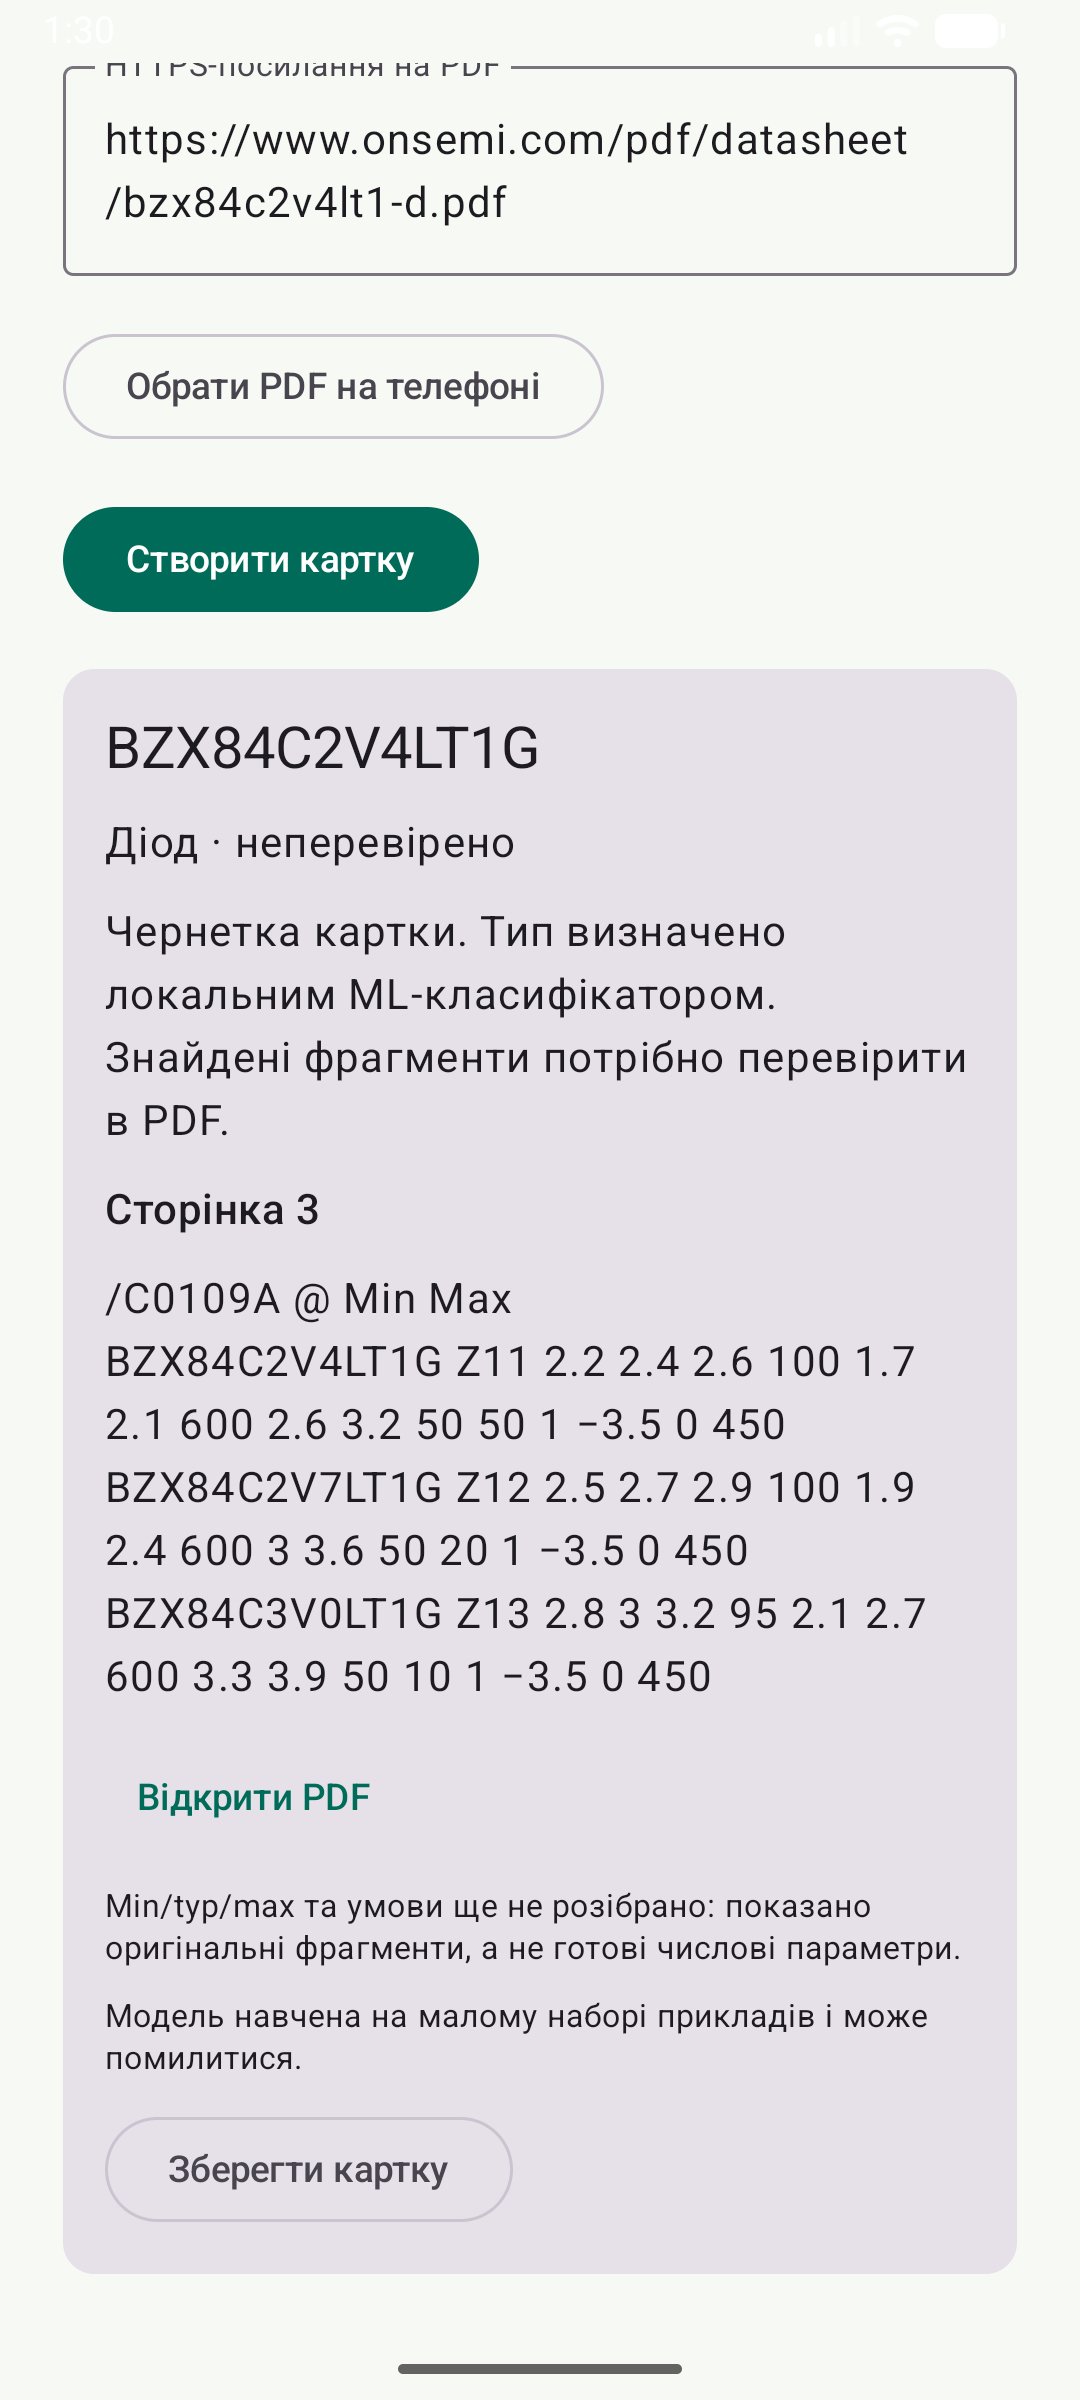
\includegraphics[width=0.65\textwidth,height=14.5cm,keepaspectratio]{s2_lab2.png}
\caption{Отримана чернетка картки даташита}
\end{figure}

\section*{Висновок}
Я реалізував і перевірив сценарій від введення даних у мобільному додатку до відповіді backend. Запит пройшов через HTTP API, класифікатор визначив тип компонента, а результат з'явився на екрані. Також перевірив повідомлення про помилку з'єднання.

\end{document}